%% This is an example first chapter.  You should put chapter/appendix that you
%% write into a separate file, and add a line \include{yourfilename} to
%% main.tex, where `yourfilename.tex' is the name of the chapter/appendix file.
%% You can process specific files by typing their names in at the 
%% \files=
%% prompt when you run the file main.tex through LaTeX.
\chapter{Specification}

The following section describes what the system does detailing its entities.

\section{Uses Case Model}

This section describes the operations of the systems as events triggered by external actors and their interrelation.

\subsection{Actors} \label{actors}

The actors of the system are the following.

\begin{description}
	\item[Sensor device] The device responsible for registering itself in the system and sending the measured observations to it.
	\item[User] A person who interacts with the public web application that shows the observations in a data visualization.
\end{description}

\subsection{Use Cases}

\begin{figure}[ht]
	\centering
	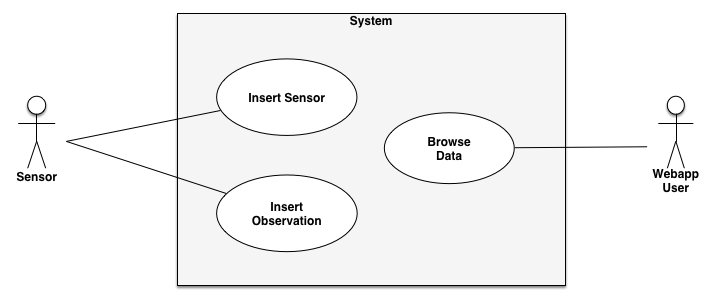
\includegraphics[width=\textwidth]{uses_cases}
	\caption{System's use cases}
	\label{fig:use_cases}
\end{figure}

\begin{usecase}
	\addtitle{Use Case 1}{Insert Sensor}
	\addfield{Actors:}{Sensor device}
	\addfield{Preconditions:}{The system is running}
	\addfield{Postconditions:}{The sensor is registered and persisted in the system}
	\addscenario{Main Success Scenario:}{
		\item The sensor sends a request to register itself
		\item The system stores the sensor's information in the database
		\item The system notifies the sensor that it has been successfully registered
	}
	\addscenario{Extensions:}{
		\item[1.a] The sensor is already registered
			\begin{enumerate}
			\item[1.] The system returns an error response
			\end{enumerate}
	}
\end{usecase}

\begin{usecase}
	\addtitle{Use Case 2}{Insert Observation}
	\addfield{Actors:}{Sensor device}
	\additemizedfield{Preconditions:}{
		\item The system is running
		\item The sensor is registered in the system	
	}
	\additemizedfield{Postconditions:}{
		\item The observation is persisted in the system
		\item The observation is sent to the web application tier
	}
	\addscenario{Main Success Scenario:}{
		\item The sensor sends a request to store the observation
		\item The system stores the observation's data in the database
		\item The system sends the observation's data to the web application tier
		\item The system notifies the sensor the observation has been successfully stored
	}
	\addscenario{Extensions:}{
		\item[1.a] The observation's sensor is not found
			\begin{enumerate}
			\item[1.] The system returns an error response
			\end{enumerate}
	}
\end{usecase}

\begin{usecase}
	\addtitle{Use Case 3}{Browse data}
	\addfield{Actors:}{User}
	\addfield{Preconditions:}{The system is running}
	\addfield{Postconditions:}{The web application is shown}
	\addscenario{Main Success Scenario:}{
		\item The user's browser loads the web application
		\item Once loaded, the web application establishes a connection against the system
		\item The system pushes the observations to the web application as they are available
	}
\end{usecase}

\section{Conceptual Model}

As shown in figure \ref{fig:use_cases}, the system revolves around the concepts of \textit{Observation} and \textit{Sensor}. The diagram \ref{fig:conceptual_model} describes these concepts and other entities involved in the system as well as their relations, heavily based on the OGC O\&M model \cite{OM}.

To start with, an observation is an aggregation of the following six elements:

\begin{description}
\item[Feature of interest] A representation of a real-world object that carries the observed property, e.g. "Pant\`a de Sau". Hence, for an in-place instrument it would be the sensor location, whereas for a remote sensor it is the target location.
\item[Procedure] Instance of a process which has performed the observation. Even though it is usually a physical sensor, it can also be a process that leads to an observation such as a computation or the result of a post-processing.
\item[Observed property] Represent the phenomena under observation. Usually a concept of an ontology, e.g. air temperature.
\item[Phenomenon time] Time when the observation's result applies.
\item[Result time] Time when the observation's result has been created. Note these two times may be identical.
\item[Result] Result of the observation, which can be either a scalar value or a complex multi-dimensional array.
\end{description}

\begin{figure}[ht]
	\centering
	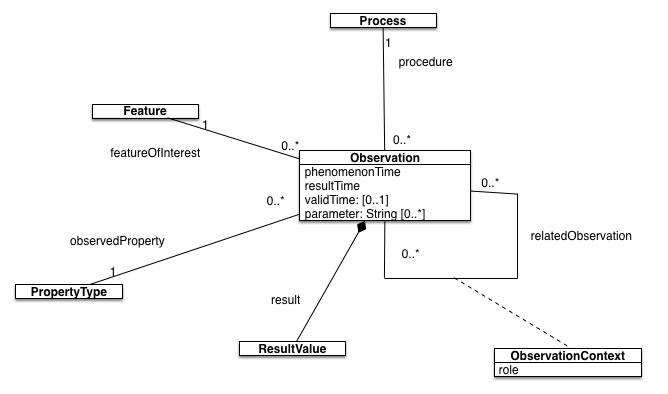
\includegraphics[width=\textwidth]{conceptual_model}
	\caption{Conceptual model}
	\label{fig:conceptual_model}
\end{figure}
\newpage

\section{Sequence Diagrams}

\begin{figure}[ht]
	\centering
	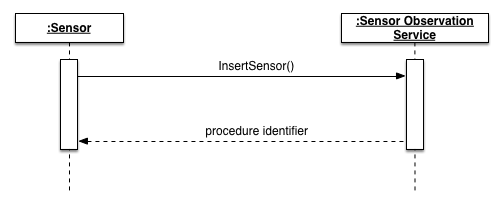
\includegraphics[scale=.75]{insert_sensor_seq}
	\caption{Sequence Diagram - Insert Sensor}
	\label{fig:insert_sensor_seq}
\end{figure}

\begin{figure}[ht]
	\centering
	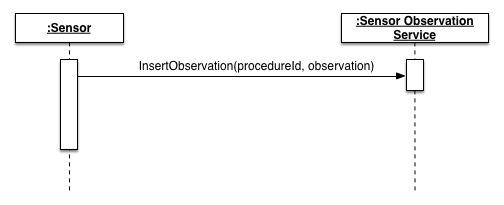
\includegraphics[scale=.75]{insert_observation_seq}
	\caption{Sequence Diagram - Insert Observation}
	\label{fig:insert_observation_seq}
\end{figure}

\begin{figure}[ht]
	\centering
	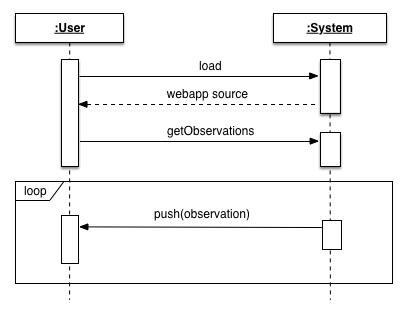
\includegraphics[scale=.75]{browse_data_seq}
	\caption{Sequence Diagram - Browse Data}
	\label{fig:browse_data_seq}
\end{figure}
